\chapter{Tuning Hadoop Cluster for Best Performance}\label{chap:7}
In this chapter, we will cover:
\begin{itemize}
  \item Benchmarking and profiling a Hadoop cluster
  \item Analyzing job history with Rumen
  \item Benchmarking a Hadoop cluster with GridMix
  \item Using Hadoop Vaidya to identify performance problems
  \item Balancing data blocks for a Hadoop cluster
  \item Choosing proper block size
  \item Using compression for input and output
  \item Configuring speculative execution
  \item Setting proper number of map and reduce slots for TaskTracker
  \item Tuning JobTracker configuration
  \item Tuning TaskTracker configuration
  \item Tuning shuffle, merge and sort parameters
  \item Configuring memory for a Hadoop cluster
  \item Setting proper number of parallel copies
  \item Tuning JVM parameters
  \item Configuring JVM reuse
  \item Configuring reducer initialization time
\end{itemize}

\section{Introduction}
Hadoop performance tuning is a challenging task, mainly due to the distributed feature of the system. The sheer number of configuration properties can tell from another perspective how complicated it is to configure a Hadoop cluster. Many of the configuration parameters have effect on the performance of the cluster. Sometimes, different settings of the properties can lead to dramatic performance differences. And some properties are more relevant and sensitive than others with regard to the performance of a Hadoop cluster.

A Hadoop cluster is composed of many components. A systematic way of performance tuning is to tune the components based on their contribution on the cluster performance. Most of the Big Data applications are I/O bound, so does Hadoop. So configurations that are closely related to I/O requests should be the first priority for performance tuning. For example, suboptimal configuration on data replication properties can cause large number of data block copies over the network, which will pose negative effect on the performance of a cluster. Similarly, improper JVM configurations can cause large data swaps for intermediate data. And unbalanced data block distribution on the DataNodes can cause the suboptimal execution of map and reduce tasks.

The first step of Hadoop performance tuning is to understand how Hadoop MapReduce works with different configuration property settings. Based on this, optimized configurations or best practices can be derived. But this is not a trivial task. It requires techniques such as data collection by running controlled experiments under different parameter settings, data analysis using optimization techniques and analytical and reasoning skills. As a matter of fact, due to the challenges and novelty, Hadoop cluster performance tuning, the research community has recent projects and publications about learning and tuning the performance of a Hadoop cluster (for example, the starfish project at \url{http://www.cs.duke.edu/starfish/}).

While the method of finding the optimal parameter configurations is straightforward for tuning the performance of a Hadoop cluster, the implementation is demanding both theoretically and in practice. Various tools and strategies for optimizing Hadoop performance have been developed and adopted by the Hadoop community. For example, balancer is a tool used for balancing skewed data blocks and speculative execution is a strategy for launching a speculative task for a slowly progressing task.

In this chapter, we will introduce the following topics in general:
\begin{itemize}
  \item Identifying the performance problems by benchmarking a Hadoop cluster
  \item Tuning Hadoop configuration parameters for best performance and
  \item Using strategies and tools for Hadoop best performance tuning
\end{itemize}
Optimal settings for different Hadoop clusters can be different. In other words, the optimal configuration for one cluster might not be optimal for another cluster under different hardware configurations. So, to find the optimal settings for a specific cluster, real field work is needed.

\section{Benchmarking and profiling a Hadoop cluster}
Benchmarking of a Hadoop cluster is the first step to tune the performance of a Hadoop cluster. We can also use Hadoop benchmarks to identify configuration problems and use it as reference for performance tuning. For example, by comparing the local benchmark with clusters with similar configurations, we can have a general understanding of the cluster performance.

Typically, we benchmark a Hadoop cluster after the cluster is newly configured before putting into service to accept jobs. Because when clients can submit jobs, the benchmarks can be perplexed by client's jobs to show the real performance of a Hadoop cluster and also the benchmark jobs can cause inconveniences for clients.

In this section, we will introduce how to benchmark and stress test a Hadoop cluster using the tests and examples package included in the Hadoop distribution. More specifically, we will test the read/write performance of the HDFS cluster. In addition, we will test the failure resilience of the MapReduce framework and the performance of the MapReduce cluster under stress.

\subsection*{Getting ready}
To get started with Hadoop cluster benchmarks, we assume that a working Hadoop cluster has been configured and all the daemons are running without any issues. We also assume that the required environment variables have been properly set in proper locations. For example, we should have \verb|HADOOP_HOME| point to the home directory of Hadoop installation and have \verb|JAVA_HOME| set in file \verb|$HADOOP_HOME/conf/hadoop-env.sh|.

Login from the Hadoop cluster administrative machine to the cluster master node with command:\\
\verb|$ ssh hduser@master|
\subsection*{How to do it...}
Use the following recipe to do HDFS benchmarks:

Test the file system with command:
\lstset{style=bashstyle}
\begin{lstlisting}
$ hadoop jar $HADOOP_HOME/hadoop-test-1.1.2.jar testfilesystem -files 10 -megaBytes 10
13/04/18 21:25:36 INFO fs.FileSystem: seed = -7801967327500182430
13/04/18 21:25:36 INFO fs.FileSystem: files = 10
13/04/18 21:25:36 INFO fs.FileSystem: megaBytes = 10
13/04/18 21:25:37 INFO fs.FileSystem: creating control file: 10485760 bytes, 10 files
13/04/18 21:25:38 INFO fs.FileSystem: created control file for: 11691305 bytes
13/04/18 21:25:38 WARN mapred.JobClient: Use GenericOptionsParser for parsing the arguments. Applications should implement Tool for the same.
...
\end{lstlisting}
If there are no errors, then the test is considered successful.

Benchmark distributed write consistency on the distributed file system with command:
\lstset{style=bashstyle}
\begin{lstlisting}[language=bash]
$ hadoop jar $HADOOP_HOME/ adoop-test-*.jar DistributedFSCheck -write -nrFiles 10 -fileSize 50
\end{lstlisting}
This command will write 10 (controlled by the \verb|-nrFiles| option) files of 50MB (controlled by the \verb|-fileSize| option) with random content to the HDFS file system. It will generate a result file named \verb|TestDFSIO_results.log| with the following content:
\lstset{style=bashstyle}
\begin{lstlisting}
----- TestDFSIO ----- : write
           Date & time: Mon Apr 01 18:25:12 EDT 2013
       Number of files: 10
Total Mbytes processed: 500
     Throughput mb/sec: 8.585459665510491
Average IO rate mb/sec: 9.46606731414795
 IO rate std deviation: 2.906442884562995
Test exec time sec: 42.338
\end{lstlisting}

Similarly, we can benchmark distributed read consistency on the distributed file system with command:
\lstset{style=bashstyle}
\begin{lstlisting}[language=bash]
$ hadoop jar $HADOOP_HOME/hadoop-test-*.jar DistributedFSCheck -read -nrFiles 10 -fileSize 50
\end{lstlisting}

The command will read 10 files with size 50 from the cluster and generate a result file with the following content:
\lstset{style=bashstyle}
\begin{lstlisting}
----- TestDFSIO ----- : read
           Date & time: Mon Apr 01 18:26:13 EDT 2013
       Number of files: 10
Total MBytes processed: 500
     Throughput mb/sec: 15.531809145129225
Average IO rate mb/sec: 17.578426361083984
 IO rate std deviation: 6.313778174121274
    Test exec time sec: 42.205
\end{lstlisting}

From the output of the two (read/write consistency check) commands, we know that writing is more expensive than reading for the HDFS cluster. This is because the write operations involve more operations such as computing and recording the checksums of the data blocks etc.

The following recipe can be used to benchmark a MapReduce cluster:

Benchmark MapReduce jobs with command:
\verb|$ hadoop jar $HADOOP_HOME/hadoop-test-*.jar mapredtest 5 1000|

The mapredtest benchmark does a load test on the MapReduce computing framework. This benchmark is done with random integers, which are generated, write to files and read back from files and tested with the original files.

Test the reliability of the MapReduce distributed computing framework with command:
\lstset{style=bashstyle}
\begin{lstlisting}
$ hadoop jar $HADOOP_HOME/hadoop-test-*.jar MRReliabilityTest -libjars $HADOOP_HOME/hadoop-examples-*.jar
\end{lstlisting}

The command will intentionally cause task and TaskTracker failures on a running job.  So during the test, we will be able to see messages like: "Killing a few tasks". A sample message will be similar to the following:
\lstset{style=bashstyle}
\begin{lstlisting}
13/04/17 17:49:22 INFO mapred.ReliabilityTest: Wed Apr 17 17:49:22 EDT 2013 Killing a few tasks
13/04/17 17:49:22 INFO mapred.ReliabilityTest: Wed Apr 17 17:49:22 EDT 2013 Killed task : attempt_201304051222_0116_m_000000_0
13/04/17 17:49:22 INFO mapred.ReliabilityTest: Wed Apr 17 17:49:22 EDT 2013 Killed task : attempt_201304051222_0116_m_000000_2
13/04/17 17:49:22 INFO mapred.ReliabilityTest: Wed Apr 17 17:49:22 EDT 2013 Killed task : attempt_201304051222_0116_m_000001_0
...
java.lang.Throwable: Child Error
        at org.apache.hadoop.mapred.TaskRunner.run(TaskRunner.java:271)
Caused by: java.io.IOException: Task process exit with nonzero status of 126.
        at org.apache.hadoop.mapred.TaskRunner.run(TaskRunner.java:258)

13/04/17 17:49:38 WARN mapred.JobClient: Error reading task outputhttp://slave1:50060/tasklog?plaintext=true&attemptid=attempt_201304051222_0119_m_000037_0&filter=stdout
13/04/17 17:49:38 WARN mapred.JobClient: Error reading task outputhttp://slave1:50060/tasklog?plaintext=true&attemptid=attempt_201304051222_0119_m_000037_0&filter=stderr
\end{lstlisting}

The failed tasks will be re-executed on a different TaskTracker. So, killing one task or a few tasks should not fail a job if the cluster is resilient to failures. If a job fails after a few killed tasks, it is possibly because MapReduce is not reliable enough or not resilient to failures and hence reliability tuning (such as by adding more computing TaskTrackers) is needed.

Benchmark MapReduce for dealing with a large number of small jobs with command: \\
\verb|$ hadoop jar $HADOOP_HOME/hadoop-test-*.jar mrbench -numRuns 20|

The mrbench execute a small job a number of times (20 in this command) and checks if these small jobs are responsive and can run efficiently on the cluster. This command will generate output similar to the following:
\lstset{style=bashstyle}
\begin{lstlisting}
DataLines       Maps    Reduces AvgTime (milliseconds)
1               2       1       45231
\end{lstlisting}
This output tells us that the average run time is about 45 seconds.

Benchmark MapReduce load generator with command:
\lstset{style=bashstyle}
\begin{lstlisting}[language=bash]
$ hadoop jar $HADOOP_HOME/hadoop-test-1.1.2.jar loadgen -m 100 -r 10 -keepmap 50 -keepred 50 -indir input -outdir output
\end{lstlisting}

The result of this command will be similar to the following:
\begin{verbatim}
Original sum: 1000
Recomputed sum: 1000
Success=true
\end{verbatim}

Do stress test with the NameNode:
\lstset{style=bashstyle}
\begin{lstlisting}[language=bash]
$ hadoop jar $HADOOP_HOME/hadoop-test-*.jar nnbench -create_write
\end{lstlisting}

We will get output similar to the following:
\lstset{style=bashstyle}
\begin{lstlisting}
-------------- NNBench -------------- :
                               Version: NameNode Benchmark 0.4
                           Date & time: 2013-04-01 18:24:10,491

                        Test Operation: create_write
                            Start time: 2013-04-01 18:22:53,382
                           Maps to run: 2
                        Reduces to run: 1
                    Block Size (bytes): 1
                        Bytes to write: 0
                    Bytes per checksum: 1
                       Number of files: 1
                    Replication factor: 1
            Successful file operations: 2

        # maps that missed the barrier: 0
                          # exceptions: 0

               TPS: Create/Write/Close: 0
Avg exec time (ms): Create/Write/Close: 30037.5
            Avg Lat (ms): Create/Write: 30030.5
                   Avg Lat (ms): Close: 6.5

                 RAW DATA: AL Total #1: 60061
                 RAW DATA: AL Total #2: 13
              RAW DATA: TPS Total (ms): 60075
       RAW DATA: Longest Map Time (ms): 60045.0
                   RAW DATA: Late maps: 0
             RAW DATA: # of exceptions: 0
\end{lstlisting}

Test the Hadoop performance with large non-splittable files:
\lstset{style=bashstyle}
\begin{lstlisting}
$ hadoop jar $HADOOP_HOME/hadoop-test-*.jar testbigmapoutput -input input -output output -create 2048
13/04/18 22:16:12 INFO mapred.BigMapOutput: Writing 2147483648 bytes to in/part-0 with minKeySize: 10 keySizeRange: 990 minValueSize: 0 valueSizeRange: 20000
13/04/18 22:17:32 INFO mapred.BigMapOutput: Created in/part-0 of size: 2048MB in 79secs
Job started: Thu Apr 18 22:17:32 EDT 2013
13/04/18 22:17:33 INFO mapred.FileInputFormat: Total input paths to process : 1
13/04/18 22:17:33 INFO net.NetworkTopology: Adding a new node: /default-rack/slave1:50010
13/04/18 22:17:33 INFO net.NetworkTopology: Adding a new node: /default-rack/slave2:50010
13/04/18 22:17:33 INFO net.NetworkTopology: Adding a new node: /default-rack/slave3:50010
...
\end{lstlisting}

Test thread map spills with command: \\
threadedmapbench is a MapReduce benchmark that compares the performance of maps with multiple spills over maps with 1 spill. The output message will be similar to the following:
\lstset{style=bashstyle}
\begin{lstlisting}
hadoop jar $HADOOP_HOME/hadoop-test-*.jar threadedmapbench
13/04/18 23:16:01 INFO mapred.ThreadedMapBenchmark: Starting the benchmark for threaded spills
ThreadedMapBenchmark.0.0.1
13/04/18 23:16:02 INFO mapred.ThreadedMapBenchmark: Generating random input for the benchmark
13/04/18 23:16:02 INFO mapred.ThreadedMapBenchmark: Total data : 128 mb
13/04/18 23:16:02 INFO mapred.ThreadedMapBenchmark: Data per map: 128 mb
13/04/18 23:16:02 INFO mapred.ThreadedMapBenchmark: Number of spills : 2
13/04/18 23:16:02 INFO mapred.ThreadedMapBenchmark: Number of maps per host : 1
13/04/18 23:16:02 INFO mapred.ThreadedMapBenchmark: Number of hosts : 1
\end{lstlisting}
Sort is a typical operation of MapReduce jobs. By sorting random data, we can peek the health of our Hadoop cluster. The following steps can be used to benchmark Hadoop sort:

Generate some random text data with command:
\lstset{style=bashstyle}
\begin{lstlisting}[language=bash]
$ hadoop jar $HADOOP_HOME/hadoop-examples-*.jar randomwriter random.writer.out
\end{lstlisting}

Sort the generated random data with command:
\lstset{style=bashstyle}
\begin{lstlisting}[language=bash]
$ hadoop jar $HADOOP_HOME/hadoop-examples-*.jar sort random.writer.out random.writer.out.sorted
\end{lstlisting}

Validate the MapReduce sort algorithm with command: \\
This command will validate the accuracy of the sort algorithm. If there is no problem on the sort algorithm, we will get the following message:
\lstset{style=bashstyle}
\begin{lstlisting}[language=bash]
$ hadoop jar $HADOOP_HOME/hadoop-test-*.jar testmapredsort -m 50 -r 5 -sortInput random.writer.out -sortOutput random.writer.out.sorted
SUCCESS! Validated the MapReduce framework's 'sort' successfully.
\end{lstlisting}

\subsection*{How it works}
We can get the usage of the Hadoop benchmark of the test package with the following command:
\lstset{style=bashstyle}
\begin{lstlisting}
$ hadoop jar $HADOOP_HOME/hadoop-test-*.jar
An example program must be given as the first argument.
Valid program names are:
  DFSCIOTest: Distributed i/o benchmark of libhdfs.
  DistributedFSCheck: Distributed checkup of the file system consistency.
  MRReliabilityTest: A program that tests the reliability of the MR framework by injecting faults/failures
  TestDFSIO: Distributed i/o benchmark.
  dfsthroughput: measure hdfs throughput
  filebench: Benchmark SequenceFile(Input|Output)Format (block,record compressed and uncompressed), Text(Input|Output)Format (compressed and uncompressed)
  loadgen: Generic map/reduce load generator
  mapredtest: A map/reduce test check.
  mrbench: A map/reduce benchmark that can create many small jobs
  nnbench: A benchmark that stresses the namenode.
  testarrayfile: A test for flat files of binary key/value pairs.
  testbigmapoutput: A map/reduce program that works on a very big non-splittable file and does identity map/reduce
  testfilesystem: A test for FileSystem read/write.
  testipc: A test for ipc.
  testmapredsort: A map/reduce program that validates the map-reduce framework's sort.
  testrpc: A test for rpc.
  testsequencefile: A test for flat files of binary key value pairs.
  testsequencefileinputformat: A test for sequence file input format.
  testsetfile: A test for flat files of binary key/value pairs.
  testtextinputformat: A test for text input format.
  threadedmapbench: A map/reduce benchmark that compares the performance of maps with multiple spills over maps with 1 spill
\end{lstlisting}

We can get the usage for the testfilesystem benchmark with the following command:
\lstset{style=bashstyle}
\begin{lstlisting}
$ hadoop jar $HADOOP_HOME/hadoop-test-1.1.2.jar testfilesystem
Usage: TestFileSystem -files N -megaBytes M [-noread] [-nowrite] [-noseek] [-fastcheck]
The following table shows the meaning of each option of this benchmark command:
Option	Description
-files	Number of files to generate for the benchmark.
-megaBytes	Size in megabytes of the generated files.
-noread	Disable the data reading test.
-nowrite	Disable the data writing test.
-noseek	Disable the seek test.
-fastcheck	Whether to use fast check or not. If the value is true, the test buffer will be filled with the same value, otherwise random numbers are generated for each location in the test buffer.
\end{lstlisting}

We can get the help for the mrbench benchmark with command:
\lstset{style=bashstyle}
\begin{lstlisting}
$ hadoop jar $HADOOP_HOME/hadoop-test-*.jar mrbench --help
MRBenchmark.0.0.2
Usage: mrbench [-baseDir <base DFS path for output/input, default is /benchmarks/MRBench>]
          [-jar <local path to job jar file containing Mapper and Reducer implementations, default is current jar file>]
          [-numRuns <number of times to run the job, default is 1>]
          [-maps <number of maps for each run, default is 2>]
          [-reduces <number of reduces for each run, default is 1>]
          [-inputLines <number of input lines to generate, default is 1>]
          [-inputType <type of input to generate, one of ascending (default), descending, random>]
          [-verbose]
\end{lstlisting}

We can get the usage of the loadgen benchmark with command:
\lstset{style=bashstyle}
\begin{lstlisting}
$ hadoop jar $HADOOP_HOME/hadoop-test-*.jar loadgen
Usage: [-m <maps>] [-r <reduces>]
       [-keepmap <percent>] [-keepred <percent>]
       [-indir <path>] [-outdir <path]
       [-inFormat[Indirect] <InputFormat>] [-outFormat <OutputFormat>]
       [-outKey <WritableComparable>] [-outValue <Writable>]
\end{lstlisting}

We can get the usage for nnbench with command:
\lstset{style=bashstyle}
\begin{lstlisting}
hadoop jar softwares/hadoop/hadoop-test-*.jar nnbench
NameNode Benchmark 0.4
Usage: nnbench <options>
Options:
        -operation <Available operations are create_write open_read
         rename delete. This option is mandatory>
         * NOTE: The open_read, rename and delete operations assume that
         the files they operate on, are already available. The
         create_write operation must be run before running the other
         operations.
        -maps <number of maps. default is 1. This is not mandatory>
        -reduces <number of reduces. default is 1. This is not mandatory>
        -startTime <time to start, given in seconds from the epoch.
         Make sure this is far enough into the future, so all maps
         (operations) will start at the same time>. default is launch
         time + 2 mins. This is not mandatory
        -blockSize <Block size in bytes. default is 1. This is not
         mandatory>
        -bytesToWrite <Bytes to write. default is 0. This is not
         mandatory>
        -bytesPerChecksum <Bytes per checksum for the files. default is 1.
         This is not mandatory>
        -numberOfFiles <number of files to create. default is 1. This is
         not mandatory>
        -replicationFactorPerFile <Replication factor for the files.
         default is 1. This is not mandatory>
        -baseDir <base DFS path. default is /becnhmarks/NNBench. This is
         not mandatory>
        -readFileAfterOpen <true or false. if true, it reads the file and
         reports the average time to read. This is valid with the
         open_read operation. default is false. This is not mandatory>
        -help: Display the help statement
\end{lstlisting}

The output tells us that only the -operation option is mandatory, all the others are optional.

We can get the usage for the testbigmapoutput benchmark with command:
\lstset{style=bashstyle}
\begin{lstlisting}
$ hadoop jar $HADOOP_HOME/hadoop-test-*.jar testbigmapoutput
BigMapOutput -input <input-dir> -output <output-dir> [-create <filesize in MB>]
\end{lstlisting}
The \verb|-input| and \verb|-output| options are mandatory for this benchmark and \verb|-create| option, which specifies the file size that is to read created is optional.

We can get the usage of the mapredtest benchmark with command:
\lstset{style=bashstyle}
\begin{lstlisting}
$ hadoop jar $HADOOP_HOME/hadoop-test-*.jar mapredtest
Usage: TestMapRed <range> <counts>

Note: a good test will have a <counts> value that is substantially larger than the <range>
\end{lstlisting}
The \verb|<range>| option specifies the range of the integer to be generated, random integers will be generated between \verb|0| and \verb|range - 1|. The \verb|<counts>| options specifies how many random integers to generate for the benchmark, it should have a substantially larger value than the \verb|<range>| option.

We can get the usage of the testmapredsort benchmark with command:
\lstset{style=bashstyle}
\begin{lstlisting}
$ hadoop jar $HADOOP_HOME/hadoop-test-*.jar testmapredsort
sortvalidate [-m <maps>] [-r <reduces>] [-deep] -sortInput <sort-input-dir> -sortOutput <sort-output-dir>
The following table shows the meaning of the options:
Option	Description
-m	Number of mappers.
-r 	Number of reducers.
-deep	Do deep validation.
-sortInput	Directory for the input data used for sort. The specified directory must exist, otherwise the benchmark will fail.
-sortOutput	Output directory after the data specified by the -sortInput directory is sorted. The specified directory must exist, otherwise the benchmark will fail.
\end{lstlisting}
\subsection*{There's more...}
Besides the Hadoop tests package, Hadoop was shipped with an example package, which can also be used to do benchmark a Hadoop cluster. We can get all the examples benchmarks with command:
\lstset{style=bashstyle}
\begin{lstlisting}
$ hadoop jar $HADOOP_HOME/hadoop-example-*.jar
Valid program names are:
  aggregatewordcount: An Aggregate based map/reduce program that counts the words in the input files.
  aggregatewordhist: An Aggregate based map/reduce program that computes the histogram of the words in the input files.
  dbcount: An example job that count the pageview counts from a database.
  grep: A map/reduce program that counts the matches of a regex in the input.
  join: A job that effects a join over sorted, equally partitioned datasets
  multifilewc: A job that counts words from several files.
  pentomino: A map/reduce tile laying program to find solutions to pentomino problems.
  pi: A map/reduce program that estimates Pi using monte-carlo method.
  randomtextwriter: A map/reduce program that writes 10GB of random textual data per node.
  randomwriter: A map/reduce program that writes 10GB of random data per node.
  secondarysort: An example defining a secondary sort to the reduce.
  sleep: A job that sleeps at each map and reduce task.
  sort: A map/reduce program that sorts the data written by the random writer.
  sudoku: A sudoku solver.
  teragen: Generate data for the terasort
  terasort: Run the terasort
  teravalidate: Checking results of terasort
  wordcount: A map/reduce program that counts the words in the input files.
\end{lstlisting}

Some commands are very handy for testing the configuration of a Hadoop cluster. For example, we can use the following command to test the cluster by computing $\pi$ (pi): \\
\verb|$ hadoop jar $HADOOP_HOME/hadoop-example-*.jar pi 10 1000000| \\
This command will start a MapReduce job to compute $\pi$ with 10 mappers with each mapper generating 1000000 samples.

The usage for randomwriter is as follows:
\lstset{style=bashstyle}
\begin{lstlisting}[language=bash]
$ hadoop jar $HADOOP_HOME/hadoop-example-*.jar randomwriter <out-dir>
\end{lstlisting}
\verb|<out-dir>| specifies the output directory of randomwriter.

The usage for sort is as follows: 
\lstset{style=bashstyle}
\begin{lstlisting}
$ sort [-m <maps>] [-r <reduces>] [-inFormat <input format class>] [-outFormat <output format class>] [-outKey <output key class>] [-outValue <output value class>] [-totalOrder <pcnt> <num samples> <max splits>] <input> <output>
\end{lstlisting}

The meaning of each option is shown in the following table:
\begin{table}[ht]
  \centering
  \begin{tabular}{ll}
    \toprule
    \textbf{Option} & \textbf{Description} \\ \midrule
      -m & Number of map tasks \\
      -r & Number of reduce tasks \\
      -inFormat & Input format class \\
      -outFormat & Output format class \\
      -outKey & Output key class \\
      -outValue & Output value class \\
      -totalOrder & \begin{minipage}[t]{0.8\textwidth}Specifies to use the TotalOrderPartitioner to partition the input data. Three parameters are needed: \verb|<pcnt>| specifies the number of partitions, \verb|<num samples>| specifies the number of samples and \verb|<max splits>| specifies the maximum number of splits for the data.\end{minipage} \\
      input & Sort input directory \\
      output & Sort output directory \\ \bottomrule
    \end{tabular}
    \caption{Options for the sort example.}\label{tbl:sort}
  \end{table}

The usage for wordcount is as follows:
\lstset{style=bashstyle}
\begin{lstlisting}[language=bash]
$ hadoop jar $HADOOP_HOME/hadoop-example-*.jar wordcount <in> <out>
\end{lstlisting}
\verb|<in>| specifies the directory for input and \verb|<out>| specifies the directory for output.

\subsection*{See also}
\begin{itemize}
  \item Benchmarking a Hadoop cluster with GridMix.
\end{itemize}
\section{Analyzing job history with Rumen}
Rumen is a tool for extracting well formatted information from job log files. It parses logs and generates statistics for the Hadoop jobs. The job traces can be used for performance tuning and simulation.

Current Rumen implementation includes two components, trace builder and folder. The trace builder takes job history as input and generates easily parsed json files. The folder is a utility to manipulate on input traces, and for most of the time, it is used to scale the summarized job traces from the trace builder. For example, we can use the folder tool to scale up (make time longer) or down (make time shorter) the job runtime. In this recipe, we will outline steps to analyze job history with Rumen.

\subsection*{Getting ready}
Before getting started, we assume that the Hadoop cluster has been properly configured and all the daemons are running without any issues.
Login from the Hadoop cluster administrator machine to the cluster master node with command: \\
\verb|$ ssh hduser@master|

\subsection*{How to do it...}
Use the following recipe to analyze job history with Rumen:

Use the trace builder to extract the ``Gold Trace'' from the Hadoop job history files. The syntax of the command is:
\lstset{style=bashstyle}
\begin{lstlisting}[language=bash]
$ hadoop org.apache.hadoop.tools.rumen.TraceBuilder [options] <jobtrace-output> <topology-output> <inputs>
\end{lstlisting}

For example, we can use the following command to extract job trace and topology from the job history directory:
\lstset{style=bashstyle}
\begin{lstlisting}[language=bash]$ hadoop org.apache.hadoop.tools.rumen.TraceBuilder -recursive file:///tmp/jobtraces.json file:///tmp/topology.out file:///usr/local/hadoop/logs/history/done
\end{lstlisting}

This command will recursively extract job history traces as well as the topology of the cluster from the Hadoop job history directory \verb|$HADOOP_HOME/logs/history/done|. The '\verb|-recursive|' option tells the TraceBuider to scan the job history directory recursively.

The output file jobtraces.json will contain all the metrics of MapReduce jobs similar to the following:
\lstset{style=bashstyle}
\begin{lstlisting}
{
  "priority" : "NORMAL",
  "jobID" : "job_201304012206_0001",
  "user" : "hduser",
  "jobName" : "PiEstimator",
  "mapTasks" : [ {
    "startTime" : 1364868424530,
    "attempts" : [ {
      "location" : {
        "layers" : [ "default-rack", "master" ]
      },
      "hostName" : "/default-rack/master",
      "result" : "SUCCESS",
      "startTime" : 1364868424536,
      "finishTime" : 1364868426761,
      "attemptID" : "attempt_201304012206_0001_m_000000_0",
      "shuffleFinished" : -1,
      "sortFinished" : -1,
      "hdfsBytesRead" : 242,
      "hdfsBytesWritten" : -1,
      "fileBytesRead" : -1,
      "fileBytesWritten" : 51959,
      "mapInputRecords" : 1,
      "mapOutputBytes" : 18,
      "mapOutputRecords" : 2,
      "combineInputRecords" : 0,
      "reduceInputGroups" : -1,
      "reduceInputRecords" : -1,
      "reduceShuffleBytes" : -1,
      "reduceOutputRecords" : -1,
      "spilledRecords" : 2,
      "mapInputBytes" : 24,
      "resourceUsageMetrics" : {
        "cumulativeCpuUsage" : 600,
        "virtualMemoryUsage" : 764727296,
        "physicalMemoryUsage" : 185315328,
        "heapUsage" : 173867008
      }
    } ],
    "finishTime" : 1364868426971,
    "preferredLocations" : [ {
      "layers" : [ "default-rack", "master" ]
    } ],
    "taskType" : "MAP",
    "taskStatus" : "SUCCESS",
    "taskID" : "task_201304012206_0001_m_000000",
    "inputBytes" : 242,
    "inputRecords" : 1,
...
"outputBytes" : 51959,
  "reduceTasks" : [ {
    "startTime" : 1364868426978,
    "attempts" : [ {
      "location" : {
        "layers" : [ "default-rack", "master" ]
      },
      "hostName" : "/default-rack/master",
      "result" : "SUCCESS",
      "startTime" : 1364868426995,
      "finishTime" : 1364868441901,
      "attemptID" : "attempt_201304012206_0001_r_000000_0",
      "shuffleFinished" : 1364868440476,
...
  "failedReduceAttemptCDF" : {
    "maximum" : 9223372036854775807,
    "minimum" : -9223372036854775808,
    "rankings" : [ ],
    "numberValues" : 0
  },
  "mapperTriesToSucceed" : [ 1.0 ],
  "failedMapperFraction" : 0.0,
  "relativeTime" : 0,
  "clusterMapMB" : -1,
  "clusterReduceMB" : -1,
  "jobMapMB" : 200,
  "jobReduceMB" : 200
}
\end{lstlisting}

The second step of using Rumen is to scale the data generated from the previous step. We can use the following syntax to do this:
\lstset{style=bashstyle}
\begin{lstlisting}[language=bash]
$ hadoop org.apache.hadoop.tools.rumen.Folder [options] [input] [output]
\end{lstlisting}

For example, to scale the runtime of the job trace generated in the previous step to 50 minutes, we can use the following command:
\lstset{style=bashstyle}
\begin{lstlisting}[language=bash]
$ hadoop org.apache.hadoop.tools.rumen.Folder -output-duration 50m -input-cycle 20m file:///home/hduser/jobtraces.json file:///home/hduser/job-scaled-50min.json
\end{lstlisting}

In this command, option \verb|-output-duration| defines the final runtime of the job trace, and the default value for this option is one hour. Option \verb|-input-cycle| is a mandatory option, and it defines the basic unit of time for the folding operation.
\subsection*{See also}
\begin{itemize}
  \item Benchmarking a Hadoop cluster with GridMix.
  \item \url{http://hadoop.apache.org/docs/r1.1.2/rumen.html}
  \item \url{https://issues.apache.org/jira/browse/MAPREDUCE-751}
\end{itemize}
\section{Benchmarking a Hadoop cluster with GridMix}
GridMix is a tool for benchmarking Hadoop clusters. It generates a number of synthetic MapReduce jobs and builds a model based on the performance of these jobs. Resource profiles of the cluster are modelled based on the job execution metrics. The profiles can help us find performance bottlenecks of the cluster. In this section, we will outline steps for benchmarking Hadoop with GridMix.
\subsection*{Getting ready}
We assume that our Hadoop cluster has been properly configured and all the daemons are running without any issues.

Currently, GridMix has three versions. For the purpose of differentiation and notation, we will use GridMix to represent GridMix version 1, use GridMix2 to represent GridMix version 2 and use GridMix3 to represent GridMix version 3.

Login to the Hadoop cluster node from the administrator machine with command:\\
\verb|$ ssh hduser@master|
\subsection*{How to do it...}
Use the following recipe to do GridMix2 benchmarks:

Change the current working directory with command: \\
\verb|$ cd $HADOOP_HOME/src/benchmarks/gridmix2|

Build the GridMix2 package with command: \\
\verb|$ ant|

Copy the gridmix.jar file to the current working directory with command: \\
\verb|$ cp build/gridmix.jar .|

Open file gridmix-env-2 with a text editor and change the environment variables similar to the following:
\lstset{style=bashstyle}
\begin{lstlisting}
export HADOOP_VERSION=hadoop-1.1.2
export HADOOP_HOME=/usr/local/hadoop
export HADOOP_CONF_DIR=$HADOOP_HOME/conf
export USE_REAL_DATASET=FALSE

export APP_JAR=${HADOOP_HOME}/hadoop-test-*.jar
export EXAMPLE_JAR=${HADOOP_HOME}/hadoop-examples-*.jar
export STREAMING_JAR=${HADOOP_HOME}/contrib/streaming/hadoop-streaming-*.jar
\end{lstlisting}

Open the GridMix2 configuration file \verb|gridmix_config.xml| with a text editor and change the benchmark configuration by changing the properties for the benchmark. For example, the following lines configure the number of jobs for streamSort benchmark with small jobs:
\lstset{style=bashstyle}
\begin{lstlisting}[language=XML]
<property>
  <name>streamSort.smallJobs.numOfJobs</name>
  <value>10,5</value>
</property>

<property>
  <name>streamSort.smallJobs.numOfReduces</name>
  <value>6,3</value>
</property>
\end{lstlisting}
These two properties specify that we will use 10 small stream sort job with 6 reducers and 5 small stream sort job with 3 reducers. All other configurations should follow rules similar to this one.

Make script generateGridmix2Data.sh executable with command: \\
\verb|$ chmod +x generateGridmix2Data.sh|

Generate data with command:
\lstset{style=bashstyle}
\begin{lstlisting}
./generateGridmix2Data.sh
Job started: Fri Apr 19 16:02:48 EDT 2013
Running 492 maps.
Job started: Fri Apr 19 16:02:48 EDT 2013
Running 492 maps.
Job started: Fri Apr 19 16:02:48 EDT 2013
13/04/19 16:02:49 INFO mapred.JobClient: Running job: job_201304051222_0233
13/04/19 16:02:49 INFO mapred.JobClient: Running job: job_201304051222_0234
13/04/19 16:02:49 INFO mapred.JobClient: Running job: job_201304051222_0235
...
\end{lstlisting}

\begin{info}
This command will generate data on HDFS. By default the generated data will be compressed with a block compression ratio of 4. Three jobs will be started in our example.
\end{info}

Make script \verb|rungridmix_2| to be executable with command: \\
\verb|$ chmod +x rungridmix_2|

Run the GridMix2 benchmark with command:
\lstset{style=bashstyle}
\begin{lstlisting}
./rungridmix_2

Jobs in waiting state: 30
Jobs in ready state: 0
Jobs in running state: 140
Jobs in success state: 32
Jobs in failed state: 0
\end{lstlisting}

\subsection*{How it works...}
GridMix is a benchmark for Hadoop clusters. It is generally used to model the performance profile of a Hadoop cluster by running a number of jobs.

The data required by GridMix is generated by running the generateGridmix2data.sh script. We can configure this file to change, for example, the size of the generated data file. Then, when executing script \verb|rungridmix_2|, a number of jobs will be generated and submitted in batch mode. In the end, the running time of these jobs will be computed.

GridMix2 is shipped with the following representative jobs: streamSort, javaSort, webdataSort, combiner, monsterSort. These jobs can be classified into the following categories:
\begin{itemize}
  \item Three stage MapReduce job, which is motivated by the multi-stage or pipelined MapReduce jobs
  \item Large sort of variable key/value sizes, which is motivated by the processing of large data sets
  \item Reference select job, which is motivated by jobs that sample from a large, reference data set
  \item API text sort jobs, which is motivated by the application of MapReduce APIs for sorting
\end{itemize}
A GridMix benchmark is a mix of a number of small, medium and large jobs from different categories. We can specify the mix in file \verb|gridmix_config.xml|. Based on the specification, a number of jobs will be created and submitted to the Hadoop cluster till finish.
\subsection*{There's more...}
Besides doing benchmark with \verb|GridMix2|, we can also benchmark a Hadoop cluster with \verb|GridMix1| and \verb|GridMix3|.

\subsubsection*{Benchmarking Hadoop cluster with GridMix1}
The usage of GridMix1 is similar to GridMix2. The following steps can be used:

Change to the GridMix1 directory: \\
\verb|$ cd $HADOOP_HOME/src/benchmarks/gridmix|

Open file gridmix-env with a text editor and change the configuration to the following:
\lstset{style=bashstyle}
\begin{lstlisting}
export HADOOP_HOME=/usr/local/Hadoop
export GRID_MIX_HOME=$HADOOP_HOME/src/benchmarks/gridmix
export APP_JAR=${HADOOP_HOME}/hadoop-test-*.jar
export EXAMPLE_JAR=${HADOOP_HOME}/hadoop-examples-*.jar
export STREAMING_JAR=${HADOOP_HOME}/contrib/streaming/hadoop-streaming-*.jar
export GRID_MIX_DATA=/gridmix1/data
export GRID_MIX_PROG=/gridmix1/programs
\end{lstlisting}

The last two environment variables \verb|GRID_MIX_DATA| and \verb|GRID_MIX_PROG| specify two directories on HDFS. So, the generated data and programs will be on HDFS.

Make script generateData.sh executable with command: \\
\verb|$ chmod +x generateData.sh|

Generate data with command: \\
\verb|$ sh ./generateData.sh|

\verb|GridMix1| is composed a number of high level scripts to control how benchmark jobs work. The tree structure of the GridMix1 directory is similar to the following:
%%%%% add files.

The \verb|GridMix1| directory contains a few template jobs with different sizes. For example, the three scripts (\emph{text-sort.small}, \emph{text-sort.medium} and \emph{text-sort.large}) in the javasort directory are templates for small, medium and large javasort jobs.

To run a small javasort job, we can use the following command:\\
\verb|$ sh javasort/text-sort.small|

We can use similar commands to run medium and large jobs.

\subsubsection*{Benchmarking Hadoop cluster with GridMix3}
Use the following recipe to build a GridMix3 benchmark for a Hadoop cluster:

Copy required jar files to Hadoop lib directory with commands:
\lstset{style=bashstyle}
\begin{lstlisting}[language=bash]
$ cp $HADOOP_HOME/hadoop-tools-*.jar $HADOOP_HOME/lib
$ cp $HADOOP_HOME/contrib/gridmix/hadoop-gridmix-*.jar $HADOOP_HOME/lib
\end{lstlisting}

File \verb|hadoop-tools-*.jar| contains tools such as Rumen, which is needed by GridMix3. And file \verb|hadoop-gridmix-*.jar| contains the GridMix3 benchmark tool. In addition, the GridMix3 job mix for a Hadoop cluster is typically described with a job trace file, which is generated from job configuration files using Rumen.

Use Rumen to generate job trace file with command:
\lstset{style=bashstyle}
\begin{lstlisting}[language=bash]
$ hadoop org.apache.hadoop.tools.rumen.TraceBuilder -recursive file:///tmp/jobtrace.json file:///tmp/topology.out file:///usr/local/hadoop/logs/history/done
\end{lstlisting}

The command will generate job trace file \verb|/tmp/jobtrace.json|, and in the next step, we are going to use this file as input for the GridMix3 Hadoop benchmarks.

Sometimes, we might get CRC exception when running this command. A quick fix for this problem is to delete the .crc file for the corresponding job configuration file.  For example, the checksum file for job configuration file \verb|job_201304051222_0192_conf.xml| is \verb|job_201304051222_0192_conf.xml.crc|, we can delete the latter file to ignore the \verb|.crc| check.

Run GridMix3 benchmark with command:
\lstset{style=bashstyle}
\begin{lstlisting}
$ hadoop org.apache.hadoop.mapred.gridmix.Gridmix -generate 100m gridmixdata  /tmp/jobtraces.json
13/04/01 22:57:11 INFO gridmix.SubmitterUserResolver:  Current user resolver is SubmitterUserResolver
13/04/01 22:57:11 INFO gridmix.Gridmix:  Submission policy is STRESS
13/04/01 22:57:11 INFO util.NativeCodeLoader: Loaded the native-hadoop library
13/04/01 22:57:11 WARN snappy.LoadSnappy: Snappy native library not loaded
13/04/01 22:57:11 INFO gridmix.CompressionEmulationUtil: GridMix is configured to generate compressed input data with  a compression ratio of 0.5
13/04/01 22:57:11 INFO gridmix.Gridmix: Generating 100.0m of test data...
13/04/01 22:57:11 INFO gridmix.Statistics: Not tracking job GRIDMIX_GENERATE_INPUT_DATA as seq id is less than zero: -1
\end{lstlisting}

To get the usage and available parameters for GridMix3, we can use the following command:
\lstset{style=bashstyle}
\begin{lstlisting}
hadoop org.apache.hadoop.mapred.gridmix.Gridmix
The general command line syntax is
bin/hadoop command [genericOptions] [commandOptions]

Usage: gridmix [-generate <MiB>] [-users URI] [-Dname=value ...] <iopath> <trace>
  e.g. gridmix -generate 100m foo - Configuration parameters:
   General parameters:
       gridmix.output.directory               : Output directory
       gridmix.client.submit.threads          : Submitting threads
...
\end{lstlisting}
\subsection*{See also}
\begin{itemize}
  \item Benchmarking and profiling a Hadoop cluster
  \item \url{http://hadoop.apache.org/docs/r1.1.2/rumen.html}
  \item \verb|$HADOOP_HOME/src/benchmarks/README.gridmix2|
\end{itemize}

\section{Using Hadoop Vaidya to identify performance problems}
Hadoop Vaidya is an open source, rule based performance diagnostic framework for Apache Hadoop. Each rule can identify a specific performance problem. For example, Hadoop cluster administrators can use Vaidya to identify slow progressing jobs that are wasting cluster resources. And Hadoop clients can use Vaidya to identify configuration mistakes for their submitted jobs.

Hadoop Vaidya is extensible, users can analyze Hadoop job with their own rules. In this recipe, we will outline steps to configure Hadoop Vaidya for Hadoop cluster performance diagnosis.

\subsection*{Getting ready}
Before getting started, we assume that the Hadoop cluster has been properly configured and all the daemons are running without any issues.

Login from the Hadoop cluster administrator machine to the master node machine with command:\\
\verb|$ ssh hduser@master|
\subsection*{How to do it...}
Use the following steps to use Hadoop Vaidya: \\
Locate the directory for the job configuration file you want to analyze. The default location of this folder is \verb|$HADOOP_HOME/logs|.

Locate the job history files under the job history directory with command:\\
\verb|$ find $HADOOP_HOME/logs -name 'job_201304012330_0001*'| \\

This command assumes that at least one job has been run so that at least one job configuration file can be found. For purpose of illustration, we assume that a teragen job has finished before running this command.

For example, in this command, we want to get the configuration file for job with JobID \verb|job_201304012330_0001|. We can get the following two lines as output:
\lstset{style=bashstyle}
\begin{lstlisting}
logs/history/job_201304012330_0001_conf.xml
logs/history/job_201304012330_0001_1364874504561_hduser_TeraGen
\end{lstlisting}
The first xml file in the output is the job configuration file and the second one is the job log file.

Use Vaidya to analyze the job trace files with command:
\lstset{style=bashstyle}
\begin{lstlisting}[language=bash]
$ sh $HADOOP_HOME/contrib/vaidya/bin/vaidya.sh -jobconf file:///usr/local/hadoop/logs/history/job_201304012330_0002_conf.xml -joblog file:///usr/local/hadoop/logs/history/job_201304012330_0002_1364874504561_hduser_TeraGen -report report.txt
\end{lstlisting}

\begin{info}
Note that the file location should be an absolute path including the schema, which is either \verb|hdfs://| or \verb|file://|.
\end{info}

This command will generate file report.txt with content similar to the following:
\lstset{style=bashstyle}
\begin{lstlisting}[language=XML]
<?xml version=''1.0'' encoding=''UTF-8'' standalone=''no''?>
<PostExPerformanceDiagnosticReport>
    <JobInformationElement>
        <JobTrackerID/>
        <JobName>PiEstimator</JobName>
        <JobType>MAP_REDUCE</JobType>
        <User>hduser</User>
        <SubmitTime>2013-04-17 19:46:49.213</SubmitTime>
        <LaunchTime>2013-04-17 19:46:49.369</LaunchTime>
        <FinishTime>2013-04-17 19:54:06.833</FinishTime>
        <Status>SUCCESS</Status>
    </JobInformationElement>
    <TestReportElement>
        <TestTitle>Balanaced Reduce Partitioning</TestTitle>
        <TestDescription>This rule tests as to how well the input to reduce tasks is balanced</TestDescription>
        <TestImportance>HIGH</TestImportance>
        <TestResult>NEGATIVE(PASSED)</TestResult>
        <TestSeverity>0.0</TestSeverity>
        <ReferenceDetails>
          * TotalReduceTasks: 1
          * BusyReduceTasks processing 0.85% of total records: 1
          * Impact: 0.0</ReferenceDetails>
        <TestPrescription>
          * Use the appropriate partitioning function
          * For streaming job consider following partitioner and hadoop config parameters
          * org.apache.hadoop.mapred.lib.KeyFieldBasedPartitioner  
          * -jobconf stream.map.output.field.separator, -jobconf stream.num.map.output.key.fields
        </TestPrescription>
    </TestReportElement>
    <TestReportElement>
        <TestTitle>Impact of Map tasks Re-Execution</TestTitle>
        <TestDescription>This test rule checks percentage of map task re-execution impacting the job performance</TestDescription>
        <TestImportance>HIGH</TestImportance>
        <TestResult>NEGATIVE(PASSED)</TestResult>
        <TestSeverity>0.0</TestSeverity>
        <ReferenceDetails>
          * Total Map Tasks: 10
          * Launched Map Tasks: 10
          * Percent Maps ReExecuted: 0
          * Impact: 0.0
        </ReferenceDetails>
        <TestPrescription>
          * Need careful evaluation of why maps are re-executed.  
          * It could be due to some set of unstable cluster nodes.
          * It could be due application specific failures.
        </TestPrescription>
    </TestReportElement>
    <TestReportElement>
        <TestTitle>Impact of Reduce tasks Re-Execution</TestTitle>
        <TestDescription>This test rule checks percentage of reduce task re-execution impacting the job performance</TestDescription>
        <TestImportance>HIGH</TestImportance>
        <TestResult>NEGATIVE(PASSED)</TestResult>
        <TestSeverity>0.0</TestSeverity>
        <ReferenceDetails>
          * Total Reduce Tasks: 1
          * Launched Reduce Tasks: 1
          * Percent Reduce Tasks ReExecuted: 0
          * Impact: 0.0</ReferenceDetails>
        <TestPrescription>
          * Need careful evaluation of why reduce tasks are re-executed.
          * It could be due to some set of unstable cluster nodes.
          * It could be due application specific failures.
        </TestPrescription>
    </TestReportElement>
    <TestReportElement>
        <TestTitle>Map and/or Reduce tasks reading HDFS data as a side effect</TestTitle>
        <TestDescription>
        This test rule checks if map/reduce tasks are reading data from HDFS as a side effect. More the data read as a side effect can potentially be a bottleneck across parallel execution of map/reduce tasks.
        </TestDescription>
        <TestImportance>HIGH</TestImportance>
        <TestResult>POSITIVE(FAILED)</TestResult>
        <TestSeverity>0.99</TestSeverity>
        <ReferenceDetails>
          * Total HDFS Bytes read: 2440
          * Total Map Input Bytes read: 240
          * Impact: 1.0
        </ReferenceDetails>
        <TestPrescription>
          Map and/or Reduce tasks are reading application specific files from HDFS. Make sure the replication factor of these HDFS files is high enough to avoid the data reading bottleneck. Typically replication factor can be square root of map/reduce tasks capacity of the allocated cluster.
        </TestPrescription>
    </TestReportElement>
    <TestReportElement>
        <TestTitle>Map side disk spill</TestTitle>
        <TestDescription>
          This test rule checks if Map tasks are spilling the data on to the local disk during the map side sorting due to insufficient sort buffer size. The impact is calculated as ratio between local bytes written to map output bytes. Impact is normalized using NormalizationFactor given below and any value greater than or equal to normalization factor is treated as maximum (i.e. 1).
        </TestDescription>
        <TestImportance>LOW</TestImportance>
        <TestResult>POSITIVE(FAILED)</TestResult>
        <TestSeverity>0.33</TestSeverity>
        <ReferenceDetails>
          * TotalMapOutputBytes: 180
          * Total Local Bytes Written by Maps: 219400
          * Impact: 1.0</ReferenceDetails>
        <TestPrescription>
          * Use combiner to lower the map output size.
          * Increase map side sort buffer size (io.sort.mb:100).
          * Increase index buffer size (io.sort.record.percent:0) if number of Map Output Records are large.
          * Increase (io.sort.spill.percent:0), default 0.80 i.e. 80% of sort buffer size and index buffer size.
        </TestPrescription>
</TestReportElement>
</PostExPerformanceDiagnosticReport>
\end{lstlisting}
\subsection*{How it works...}
We can get the options for Vaidya with the following command:
\lstset{style=bashstyle}
\begin{lstlisting}
$ $HADOOP_HOME/contrib/vaidya/bin/vaidya.sh -help
Invalid arguments: -jobconf or -joblog arguments are missing
Usage:
PostExPerformanceDiagnoser -jobconf <fileurl> -joblog <fileurl> [-testconf <filepath>] [-report <filepath>]

-jobconf <fileurl>     : File path for job configuration file (e.g. job_xxxx_conf.xml). It can be on HDFS or
                       : local file system. It should be specified in the URL format.
                       : e.g. local file => file://localhost/Users/hadoop-user/job_0001_conf.xml
                       : e.g. hdfs file  => hdfs://namenode:port/Users/hadoop-user/hodlogs/.../job_0001_conf.xml

-joblog <fileurl>      : File path for job history log file. It can be on HDFS or local file system.
                       : It should be specified in the URL format.

-testconf <filepath>   : Optional file path for performance advisor tests configuration file. It should be available
                       : on local file system and be specified as as an absolute file path.
                       : e.g. => /Users/hadoop-user/postex_diagnosis_tests.xml. If not specified default file will be used
                       : from the hadoop-{ver}-vaidya.jar in a classpath.
                       : For user to view or make local copy of default tests, file is available at $HADOOP_HOME/contrib/vaidya/conf/postex_diagnosis_tests.xml

-report <filepath>     : Optional file path for for storing diagnostic report in a XML format. Path should be available
                       : on local file system and be specified as as an absolute file path.
                       : e.g. => /Users/hadoop-user/postex_diagnosis_report.xml. If not specified report will be printed on console

-help                  : prints this usage
\end{lstlisting}
\subsection*{There's more...}
HiBench is a benchmarking suite for Hadoop. It has 9 typical workloads, including micro, HDFS, web search machine learning and data analytics benchmarks. For example, it supports benchmarks for Nutch (a text indexing software package), PageRank (the PageRank algorithm), the Mahout machine learning algorithms and Hive queries.
The HiBench project and the paper provide nice examples of Hadoop benchmarking. For more information, you can refer to: \url{https://github.com/intel-hadoop/Hibench}.
\subsection*{See also}
\begin{itemize}
  \item Benchmarking and profiling a Hadoop cluster
  \item Benchmarking a Hadoop cluster with GridMix
  \item \url{http://hadoop.apache.org/docs/stable/vaidya.html}
\end{itemize}
\section{Balancing data blocks for a Hadoop cluster}
HDFS stores data blocks on DataNode machines. When Hadoop processes jobs, data is generated and deleted. Overtime, some DataNodes can host much more data blocks than others. This unbalanced distribution of data on the cluster is called data skew.

Data skew is a big problem for a Hadoop cluster. We know that when the JobTracker assigns tasks to TaskTrackers, it follows the general rule of being 'data local', which means the map tasks will be assigned to those hosts where data blocks reside in. If the data block storage distribution is skewed, or in other words, the data blocks locate only on a small percentage of DataNodes, only those nodes with data blocks can follow the 'data local' rule. And if JobTracker assigns tasks to other nodes that does not have data hosted locally, the data needs to be transferred from remote machines to the TaskTracker machine. The data transfer will cost large amount of network bandwidth, downgrading the overall performance of the cluster.

To deal with the data skew problem on HDFS, Hadoop is shipped with a balancer tool. It can be configured either manually or automatically to re-balance the data blocks.
\subsection*{Getting ready}
To get started with balancer, we assume that the Hadoop cluster has been properly configured and all the daemons are running without any issues.
Login from the cluster administrator machine to the master node with the following command: \\
\verb|$ ssh hduser@master|
\subsection*{How to do it...}
Use the following recipe to balance HDFS data blocks with balancer:

Check the data skew through the web UI, for example, by opening URL \url{http://master:50070/}

The webpage will be similar to Figure \ref{fig:skewed.datanode}.
\begin{figure}[ht]
  \centering
  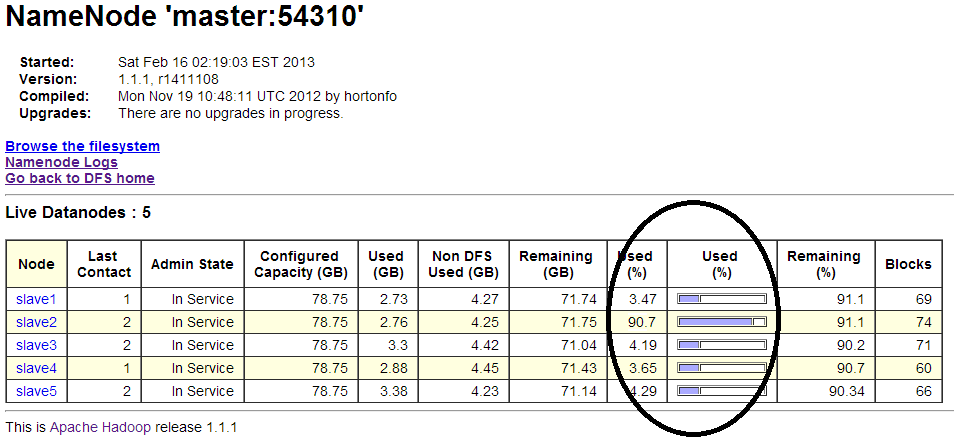
\includegraphics[width=.8\textwidth]{figs/5163os_07_01.png}
  \caption{The Skewed Datanode}\label{fig:skewed.datanode}
\end{figure} 
The screenshot shows that the data blocks are skewed. Hence, rebalancing is necessary.

Use the following command to balance the data blocks on the DataNode machines: \\
\verb|$ hadoop balancer -threshold 0.2| \\
This command will take some time to finish depending on the status of the distributed filesystem as well as the value for option \verb|-threshold|. The option \verb|-threshold| specifies the threshold for whether the cluster is balanced. It is a real number within range $[0, 1]$ with a default value 0.1. Smaller value for this option leads to more even distribution of the data blocks. On the other hand, it will require more time to finish. Setting this option to be 0 is not recommended, because it is not practical to achieve an ideal balance.

Alternatively, we can start the Hadoop balancer daemon to automatically balance the data blocks on HDFS. We can use the following command to do this: \\
\verb|$ start-balancer.sh|

The balancer will move data blocks among the DataNodes according to the space utilization. For example, it will move data blocks from high utilized nodes to the low utilized nodes. This process is done iteratively. We can get the updated DataNode information from the NameNode after each iteration. If the cluster is already balanced, we will get output similar to the following:
\lstset{style=bashstyle}
\begin{lstlisting}
Time Stamp               Iteration#  Bytes Already Moved  Bytes Left To Move  Bytes Being Moved
13/04/02 00:56:27 INFO net.NetworkTopology: Adding a new node: /default-rack/127.0.0.1:50010
13/04/02 00:56:27 INFO balancer.Balancer: 0 over utilized nodes:
13/04/02 00:56:27 INFO balancer.Balancer: 1 under utilized nodes:  127.0.0.1:50010
The cluster is balanced. Exiting...
Balancing took 567.0 milliseconds
\end{lstlisting}

To stop the balancer, we can use the following command:\\
\verb|$ stop-balancer.sh|

\subsection*{How it works}
Hadoop balancer balances data blocks on HDFS according to a pre-configured threshold value, which sets the target for whether the cluster is balanced or not. A node is considered balanced if the difference between space utilization of the node and space utilization of the cluster is less than the threshold.

Sometimes, we want to limit the percentage of bandwidth used by the balancer. By default, Hadoop defines a property dfs.balance.bandwidthPerSec, which determines the maximum speed that a data block will be moved from one DataNode to another. Its default value is 1MB/s. By configuring this property to be a higher value, the balancing speed will be faster but the more resources will be used. For example, to change the value of this property to be 10MB/s, we can open file \verb|$HADOOP_HOME/conf/hdfs-site.xml| and add the following lines:
\lstset{style=bashstyle}
\begin{lstlisting}[language=XML]
<property>
  <name>dfs.balance.bandwidthPerSec</name>
  <value>10485760</value>
</property>
\end{lstlisting}
\begin{info}We need to restart HDFS to make this change take effect.\end{info}

\section{Choosing proper block size}
HDFS stores data as data blocks distributed on multiple machines. So, when a large file put onto HDFS, it will first be splitted into a number of data blocks. These data blocks are then distributed by the NameNode to the DataNodes in the cluster. The granularity of the data blocks can affect the distribution and parallel execution of the tasks.

Based on the property of the jobs being executed, one block size might result in better performance than others. We will guide you through steps to configure proper block size for the Hadoop cluster.
\subsection*{Getting ready}
We assume that the Hadoop cluster has been properly configured and all the daemons are running without any issues.

Login from the Hadoop cluster administrator machine to the master node with command: \\
\verb|$ ssh hduser@master|
\subsection*{How to do it...}
Configure the proper HDFS block size with the following recipe:

Run a typical job on the configured cluster. For example, we can run a sample terasort on the cluster with command:
\lstset{style=bashstyle}
\begin{lstlisting}[language=bash]
$ hadoop jar $HADOOP_HOME/hadoop-example-*.jar terasort input output
\end{lstlisting}

Use Rumen to generate job traces from the job history file and the job log file with command:
\lstset{style=bashstyle}
\begin{lstlisting}[language=bash]
$ hadoop org.apache.hadoop.tools.rumen.TraceBuilder file:///tmp/jobtraces.json file:///tmp/topology.out file:///usr/local/hadoop/logs/history/done/ job_201304012206_0002_conf.xml
\end{lstlisting}

Use GridMix3 to generate Hadoop cluster benchmark with different block sizes:
\lstset{style=bashstyle}
\begin{lstlisting}[language=bash]
$ hadoop org.apache.hadoop.mapred.gridmix.Gridmix -generate 10m input jobtraces.json
\end{lstlisting}

Now, we can find the block size that achieves the best performance. For example, by setting block size to be 64MB, we can get the best performance.

Stop the cluster with command: \\
\verb|$ stop-all.sh|

Open file \verb|$HADOOP_HOME/conf/hdfs-site.xml| with your favorite text editor and change the dfs.block.size property to be the following:
\lstset{style=bashstyle}
\begin{lstlisting}[language=XML]
<property>
  <name>dfs.block.size</name>
  <value>64</value>
</property>
\end{lstlisting}

Start the Hadoop cluster with command:\\
\verb|$ start-all.sh|

\section{Using compression for input and output}
A typical MapReduce job uses parallel mapper tasks to load data from external storage devices such as hard drives to the main memory. When a job finishes, the reduce tasks write the result data back to the hard drive. Actually, during the life cycle of a MapReduce job, many data copies between the hard drive and the main memory can happen. Sometime, the data is copied over the network from a remote node.

Copying data from and to hard drives and transfers over the network are expensive operations. To reduce the cost of these operations, Hadoop introduced compression on the data.

Data compression in Hadoop is done by a compression codec, which is a program that encodes and decodes data streams. Although compression and decompression can cause additional cost to the system, the advantages far out weight the disadvantages.

In this section, we will outline steps to configure data compression on a Hadoop cluster.

\subsection*{Getting ready}
We assume that the Hadoop cluster has been properly configured and all the daemons are running without any issues.

Login from the Hadoop cluster administrator machine to the cluster master node with command: \\
\verb|$ ssh hduser@master|

In this recipe, we assume all the property configurations will make changes in file \verb|$HADOOP_HOME/conf/mapred-site.xml|.
\subsection*{How to do it...}
Use the following recipe to configure input and output data compression for a Hadoop cluster:

Stop the cluster with command: \\
\verb|$ stop-all.sh|

Enable output compression by adding the following property:
\lstset{style=bashstyle}
\begin{lstlisting}[language=XML]
<property>
  <name>mapred.output.compress</name>
  <value>true</value>
</property>
\end{lstlisting}

Specify output compression codec by changing the following property:
\lstset{style=bashstyle}
\begin{lstlisting}[language=XML]
<property>
  <name>mapred.output.compression.codec</name>
  <value>org.apache.hadoop.io.compress.GzipCodec</value>
</property>
\end{lstlisting}

The property specifies Hadoop to use Gzip codec for data compression. Other available compression codecs include \verb|org.apache.hadoop.io.compress.GzipCodec| and \verb|org.apache.hadoop.io.compress.BZip2Codec| and so on. The default value for this property is \verb|org.apache.hadoop.io.compress.DefaultCodec|.

Change the output compression type for sequence file output by changing the following property:
\lstset{style=bashstyle}
\begin{lstlisting}[language=XML]
<property>
  <name>mapred.output.compression.type</name>
  <value>BLOCK</value>
</property>
\end{lstlisting}
This will change the sequence file output compression type from the default type RECORD to BLOCK. The other types are NONE and RECORD. By setting this property to be NONE, we will disable the compression of sequence file outputs. And individual record will be compressed with the RECORD compression type and a number of records will be compressed with the BLOCK compression type. Generally, the BLOCK compression type is more efficient than RECORD type, so it is recommended.

Configure the map output compression by changing the following property:
\lstset{style=bashstyle}
\begin{lstlisting}[language=XML]
<property>
  <name>mapred.compress.map.output</name>
  <value>true</value>
</property>
\end{lstlisting}
This configuration will enable the map output compression. To disable it, which is the default, we can change the value to be 'false' or remove this configuration property from the configuration file.


Similar to the codec configuration for MapReduce job output, we can configuration compression codecs for map task output, the default of which is org.apache.hadoop.io.compress.DefaultCodec. For example, we can configure the map output compression to be Gzip codec by changing the property similar to the following:
\lstset{style=bashstyle}
\begin{lstlisting}[language=XML]
<property>
  <name>mapred.map.output.compression.codec</name>
  <value>org.apache.hadoop.io.compress.GzipCodec</value>
</property>
\end{lstlisting}

Copy the configuration file from the master node to all the slave nodes in the cluster with command:
\lstset{style=bashstyle}
\begin{lstlisting}[language=bash]
for host in `cat $HADOOP_HOME/conf/slaves`
do
  echo 'Copying mapred-site.xml file to host: ' $host
  scp $HADOOP_HOME/conf/mapred-site.xml $host:$HADOOP_HOME/conf/
done
\end{lstlisting}

Restart the Hadoop cluster with command: \\
\verb|$ start-all.sh|

\subsection*{How it works...}
The following table is a summary of properties for configuring Hadoop data compression:
\begin{table}[ht]
  \begin{tabular}{ll}
    \toprule
    \textbf{Property}  & \textbf{Default} \\ \midrule
      mapred.output.compress & true \\
      mapred.output.compression.type & RECORD \\
      mapred.output.compression.codec & org.apache.hadoop.io.compress.DefaultCodec \\
      mapred.compress.map.output & false \\
      mapred.map.output.compression.codec & org.apache.hadoop.io.compress.DefaultCodec \\ \bottomrule
    \end{tabular}
  \caption{Data compression parameters}\label{tbl:hdfscompression}
\end{table}

Available compression codecs are described in the following table:
\begin{table}[ht]
  \centering
  \begin{tabular}{ll}
    \toprule
    \textbf{Codec Name} & \textbf{Java Class} \\ \midrule
      DefaultCodec & org.apache.hadoop.io.compress.DefaultCodec \\
      GzipCodec & org.apache.hadoop.io.compress.GzipCodec \\
      BZip2Codec & org.apache.hadoop.io.compress.BZip2Codec \\
      SnappyCodec & org.apache.hadoop.io.compress.SnappyCodec \\
      LzoCodec & org.apache.hadoop.io.compress.LzoCodec\\ \bottomrule
  \end{tabular}
  \caption{HDFS Compression Codecs}\label{tbl:hdfscodecs}
\end{table}

\section{Configuring speculative execution}
Speculative execution is a proactive performance boosting strategy used by JobTracker to execute one task on two TaskTrackers. When either of these tasks finishes, the other task will be killed. By default, speculative execution is on.

Speculative execution can be helpful to improve the performance of MapReduce jobs by reducing the execution time for slowly progressing tasks.  For example, on heterogeneous Hadoop clusters with different hardware configurations, low performance computing nodes can greatly prolong the execution time of a MapReduce job. Speculative execution can remedy this problem by prioritizing the high performance nodes for MapReduce tasks execution. Hence, the MapReduce execution time can be shortened.

On the other hand, speculative execution can negatively affect the performance of the cluster when a lot of resources are used for speculative execution. For example, many tasks will have to wait for slots that are used for speculative execution.

In this recipe, we will list steps to configure Hadoop speculative execution.

\subsection*{Getting ready}
We assume that the Hadoop cluster has been properly configured and all the daemons are running without any issues.

Login from the Hadoop cluster administrator machine to the cluster master node with command: \\
\verb|$ ssh hduser@master|

In this recipe, we assume all the property configurations will make changes to file \verb|$HADOOP_HOME/conf/mapred-site.xml|.
\subsection*{How to do it...}
We can use the following recipe to configure Hadoop speculative execution:

Stop the MapReduce cluster with command: \\
\verb|$ stop-mapred.sh|

Disable map task speculative execution by changing the following property:
\lstset{style=bashstyle}
\begin{lstlisting}[language=XML]
<property>
  <name>mapred.map.tasks.speculative.execution</name>
  <value>false</value>
</property>
\end{lstlisting}
By default, Hadoop speculative execution is turned on.


Disable the reduce task speculative execution by changing the following property:
\lstset{style=bashstyle}
\begin{lstlisting}[language=XML]
<property>
  <name>mapred.reduce.tasks.speculative.execution</name>
  <value>false</value>
</property>
\end{lstlisting}


Configure the maximum percentage of concurrently running speculative tasks by changing the following property:
\lstset{style=bashstyle}
\begin{lstlisting}[language=XML]
<property>
  <name>mapreduce.job.speculative.speculativecap</name>
  <value>0.2</value>
</property>
\end{lstlisting}
This configures, in maximum, 20\% of the tasks of a job can run speculatively.


Configure the job speculative execution threshold for slow tasks by changing the following property:
\lstset{style=bashstyle}
\begin{lstlisting}[language=XML]
<property>
  <name>mapreduce.job.speculative.slowtaskthreshold</name>
  <value>1.0</value>
</property>
\end{lstlisting}

This property is used to test if a task needs to be executed speculatively. Its default value is 1.0.


Configure the threshold for a TaskTracker to speculatively execute slow tasks by changing the following property:
\lstset{style=bashstyle}
\begin{lstlisting}[language=XML]
<property>
  <name>mapreduce.job.speculative.slownodethreshold</name>
  <value>1.0</value>
</property>
\end{lstlisting}
This property is used to test if a TaskTracker is qualified to run speculative tasks. Its default value is 1.0.


Sync the configurations to the slave nodes with command:
\lstset{style=bashstyle}
\begin{lstlisting}[language=bash]
for host in `cat $HADOOP_HOME/conf/slaves`; do
  echo 'Copying mapred-site.xml file to host: ' $host
  sudo scp $HADOOP_HOME/conf/mapred-site.xml $host:$HADOOP_HOME/conf/
done
\end{lstlisting}

Started the MapReduce cluster with the following command:\\
\verb|$ start-mapred.sh|

\subsection*{How it works...}
When speculative execution is enabled, some tasks will get killed. This can be verified by opening URL: \url{http://master:50030/}.

The web page will be similar to Figure \ref{fig:killed.jobs.speculative}.
\begin{figure}[ht]
  \centering
  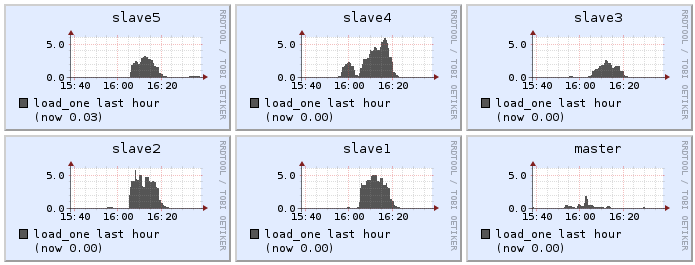
\includegraphics[width=.8\textwidth]{figs/5163os_06_10.png}
  \caption{Killed Attempts due to Speculative Execution}\label{fig:killed.jobs.speculative}
\end{figure} 
If speculative execution has been enabled for a Hadoop cluster, we can still disable it for specific jobs. For example, when we write MapReduce jobs using Java programming language, we can use the following code snippet to disable speculative execution for this job:
\lstset{style=bashstyle}
\begin{lstlisting}
Configuration conf = new Configuration();
conf.set("mapred.map.tasks.speculative.execution", "false");
conf.set("mapred.reduce.tasks.speculative.execution", "false");
\end{lstlisting}

The following table is a summary of the properties we used in this recipe with their default values:
\begin{table}[ht]
  \centering
  \begin{tabular}{ll}
    \toprule
    \textbf{Property} & \textbf{Default value} \\ \midrule
      mapreduce.map.speculative & true \\
      mapreduce.reduce.speculative & true \\
      mapreduce.job.speculative.speculativecap & 0.1 \\
      mapreduce.job.speculative.slowtaskthreshold & 1.0 \\
      mapreduce.job.speculative.slownodethreshold & 1.0 \\ \bottomrule
  \end{tabular}
  \caption{Hadoop Speculative Execution properties}\label{tbl:speculative}
\end{table}

The three properties mapreduce.job.speculative.speculativecap, \emph{mapreduce.job.speculative.slowtaskthreshold} and \emph{mapreduce.job.speculative.slownodethreshold} control when the JobTracker should start a speculative task. Specifically, a speculative task for a regular task will be started if the following conditions are met:
\begin{itemize}
  \item Speculative execution is enabled
  \item The completion rate, in percentage, of the regular task is less than \verb|mapreduce.job.speculative.slowtaskthreshold| times the mean completion rate of all other tasks.
  \item The completion rate, in percentage, of the regular task is less than \verb|mapreduce.job.speculative.slownodethreshold| times the mean completion rate of all other tasks on the current TaskTracker.
  \item The number of launched speculative tasks is smaller than the configured speculative cap.
\end{itemize}
\section{Setting proper number of map and reduce slots for TaskTracker}
The number of map and reduce slots determines the number of concurrent map/reduce tasks for a TaskTracker, which forks multiple JVMs to run these tasks. In this recipe, we will give general
\subsection*{Getting ready}
We assume that the Hadoop cluster has been properly configured and all the daemons are running without any issues.

Login from the Hadoop cluster administrator machine to the cluster master node with command: \\
\verb|$ ssh hduser@master|
\subsection*{How to do it...}
Use the following steps to configure map/reduce slots for a TaskTracker:

Stop the MapReduce cluster with command: \\
\verb|$ stop-mapred.sh|

Configure the map slots by adding the following property into file \verb|$HADOOP_HOME/conf/mapred-site.xml|:
\lstset{style=bashstyle}
\begin{lstlisting}[language=XML]
<property>
  <name>mapred.takstracker.map.tasks.maximum</name>
  <value>4</value>
</property>
\end{lstlisting}

The TaskTracker is configured to have 4 map slots.

Similarly, we can configure the number of reduce slots for a TaskTracker:
\lstset{style=bashstyle}
\begin{lstlisting}[language=XML]
<property>
  <name>mapred.takstracker.reduce.tasks.maximum</name>
  <value>4</value>
</property>
\end{lstlisting}

Configure the memory usage for each slot by adding the following property:
\lstset{style=bashstyle}
\begin{lstlisting}[language=XML]
<property>
  <name>mapred.child.java.opts</name>
  <value>-Xmx1024m</value>
</property>
\end{lstlisting}

Sync the configuration to all the slave nodes with command:
\lstset{style=bashstyle}
\begin{lstlisting}[language=bash]
for host in `cat $HADOOP_HOME/conf/slaves`; do
  echo 'Copying mapred-site.xml file to host: ' $host
  scp $HADOOP_HOME/conf/mapred-site.xml $host:$HADOOP_HOME/conf/
done
\end{lstlisting}

Start the MapReduce cluster with command: \\
\verb|$ start-mapred.sh|

\section{Tuning JobTracker configuration}
In a Hadoop cluster, the JobTracker is responsible for managing jobs and tasks. The performance of the JobTracker is critical for the whole cluster. Hadoop provides a few properties for administrators to tune the JobTracker. In this recipe, we will list the steps to configure the JobTracker.
\subsection*{Getting ready}
We assume that the Hadoop cluster has been properly configured and all the daemons are running without any issues.

Login from the Hadoop cluster administrator machine to the cluster master node with command:\\
\verb|$ ssh hduser@master|

In this recipe, we assume all the configurations are making changes to file \verb|$HADOOP_HOME/conf/mapred-site.xml|.
\subsection*{How to do it...}
Use the following recipe to configure JobTracker:

Stop the MapReduce cluster with command:\\
\verb|$ stop-mapred.sh|

Configure the maximum number of tasks for a job by changing the following property:
\lstset{style=bashstyle}
\begin{lstlisting}[language=XML]
<property>
  <name>mapred.jobtracker.maxtasks.per.job</name>
  <value>3000</value>
</property>
\end{lstlisting}
The default value of this property is -1, which ignores the limit.

Configure JobTracker to recover upon restart by changing the following property:
\lstset{style=bashstyle}
\begin{lstlisting}[language=XML]
<property>
  <name>mapred.jobtracker.restart.recover</name>
  <value>true</value>
</property>
\end{lstlisting}
By default this property is disabled, the JobTracker will start from fresh.

Configure the block size for the job history file by changing property:
\lstset{style=bashstyle}
\begin{lstlisting}[language=XML]
<property>
  <name>mapred.jobtracker.job.history.block.size</name>
  <value>3145728</value>
</property>
\end{lstlisting}

The job history data, which will be dumped to disk, will be used for job recovery.

Configure the task scheduler for the JobTracker by changing property:
\lstset{style=bashstyle}
\begin{lstlisting}[language=XML]
<property>
  <name>mapred.jobtracker.taskScheduler</name>
  <value>org.apache.hadoop.mapred.JobQueueTaskScheduler</value>
</property>
\end{lstlisting}
This configuration enables java class org.apache.hadoop.mapred.JobQueueTaskScheduler to schedule tasks.


Configure the maximum running tasks for a job by changing the following property:
\lstset{style=bashstyle}
\begin{lstlisting}[language=XML]
<property>
  <name>mapred.jobtracker.taskScheduler.maxRunningTasksPerJob</name>
  <value>20</value>
</property>
\end{lstlisting}

This property sets a limit on the maximum number of tasks for each job before it gets pre-empted by the job scheduler. It is related to the scheduling of jobs and tasks.

Sync the configuration from the master node to all the slave nodes with command:
\lstset{style=bashstyle}
\begin{lstlisting}[language=bash]
for host in `cat $HADOOP_HOME/conf/slaves`; do
  echo 'Copying mapred-site.xml file to host: ' $host
  scp $HADOOP_HOME/conf/mapred-site.xml $host:$HADOOP_HOME/conf/
done
\end{lstlisting}


Restart the Hadoop cluster with command: \\
\verb|$ start-mapred.sh|

\subsection*{How it works}
The following table is a list of properties with descriptions of this recipe:
\begin{table}[ht]
  \centering
  \begin{tabular}{lll}
    \toprule
    \textbf{Property} & \textbf{Default} & \textbf{Description} \\ \midrule
    mapred.jobtracker.maxtasks.per.job & -1 & Unlimited \\
    mapred.jobtracker.restart.recover & false & No Recover. \\
    mapred.jobtracker.job.history.block.size & 3145728 & \\
    mapred.jobtracker.taskScheduler.maxRunningTasksPerJob & EMPTY & No Limits \\ \bottomrule
  \end{tabular}
  \caption{JobTracker related configuration parameters}\label{tbl:jobtracker}
\end{table}

\subsection*{See also}
\begin{itemize}
  \item Tuning TaskTracker configuration
  \item Configuring capacity scheduler in Chapter \ref{chap:4}, Managing a Hadoop cluster
  \item Configuring fair scheduler in Chapter \ref{chap:4}, Managing a Hadoop cluster
\end{itemize}
\section{Tuning TaskTracker configuration}
TaskTrackers accept tasks from the JobTracker in a cluster and forks JVMs to run the tasks. A couple of TaskTracker properties can be configured based on the configuration of the cluster.

In this section, we will list steps to configure TaskTracker property.
\subsection*{Getting ready}
We assume that the Hadoop cluster has been properly configured and all the daemons are running without any issues.

Login from the Hadoop cluster administrator machine to the cluster master node with command: \\
\verb|$ ssh hduser@master|

In this recipe, we assume all the configurations are making changes to file \verb|$HADOOP_HOME/conf/mapred-site.xml|.
\subsection*{How to do it...}
Use the following recipe to configure TaskTracker properties:

Stop the MapReduce cluster with command: \\
\verb|$ mapred-stop.sh|

Configure the MapReduce cluster heartbeat interval by changing the following property:
\lstset{style=bashstyle}
\begin{lstlisting}[language=XML]
<property>
  <name>mapred.tasktracker.expiry.interval</name>
  <value>600000</value>
</property>
\end{lstlisting}

This property specifies the heartbeat time interval, in milliseconds, after which it will be marked lost by the JobTracker.

Configure the sleep time before sending the SIGKILL signal by changing the following property:
\lstset{style=bashstyle}
\begin{lstlisting}[language=XML]
<property>
  <name>mapred.tasktracker.tasks.sleeptime-before-sigkill</name>
  <value>6000</value>
</property>
\end{lstlisting}

This property configures the sleep time in milliseconds that the TaskTracker waits before sending a SIGKILL signal to a process after it has been sent a SIGTERM signal. Its default value is 5000ms.

Enable TaskTracker memory management by changing the following property:
\lstset{style=bashstyle}
\begin{lstlisting}[language=XML]
<property>
  <name>mapred.tasktracker.tasks.maxmemory</name>
  <value>true</value>
</property>
\end{lstlisting}

Configure the TaskTracker index cache size to be 20MB by changing the following property:
\lstset{style=bashstyle}
\begin{lstlisting}[language=XML]
<property>
  <name>mapred.tasktracker.indexcache.mb</name>
  <value>20</value>
</property>
\end{lstlisting}

This property configures the maximum memory that a TaskTracker uses for index cache when serving map output to reducers.

Configure the monitoring interval for the TaskTracker's task memory manager by changing the following property:
\lstset{style=bashstyle}
\begin{lstlisting}[language=XML]
<property>
  <name>mapred.tasktracker.taskmemorymanager.monitoring-interval</name>
  <value>5000</value>
</property>
\end{lstlisting}
This property configures the interval, in milliseconds, that the TaskTracker monitors the tasks' memory usage. It is only meaningful when tasks' memory management has been enabled using property mapred.tasktracker.tasks.maxmemory.

Configure TaskTracker to send an out-of-band heartbeat on task completion by changing the following property:
\lstset{style=bashstyle}
\begin{lstlisting}[language=XML]
<property>
  <name>mapreduce.tasktracker.outofband.heartbeat</name>
  <value>true</value>
</property>
\end{lstlisting}

The default value for this property is false, which disables the out-of-band heartbeat. Enabling this property can achieve better latency.

Configure the maximum number of retries for a map task by changing the following:
\lstset{style=bashstyle}
\begin{lstlisting}[language=XML]
<property>
  <name>mapred.map.max.attempts</name>
  <value>4</value>
</property>
\end{lstlisting}

By this configuration, a failed task will be retried up to 3 times before being declared failed.

Configure the maximum number of retries for a failed reduce task by changing the following:
\lstset{style=bashstyle}
\begin{lstlisting}[language=XML]
<property>
  <name>mapred.reduce.max.attempts</name>
  <value>4</value>
</property>
\end{lstlisting}
Similar to the max attempts configuration for a map task, this property configures to retry a failed reduce task up to 3 times before declaring failed.

Sync the configuration from the master node to all the slave nodes with command:
\lstset{style=bashstyle}
\begin{lstlisting}[language=bash]
for host in `cat $HADOOP_HOME/conf/slaves`; do
  echo 'Copying mapred-site.xml file to host: ' $host
  scp $HADOOP_HOME/conf/mapred-site.xml $host:$HADOOP_HOME/conf/
done
\end{lstlisting}

Restart the MapReduce cluster with the following command: \\
\verb|$ start-mapred.sh|

\subsection*{How it works}
The following table contains a list of properties with descriptions of this recipe:
\begin{table}[ht]
  \centering
  \begin{tabular}{lll}
    \toprule
    \textbf{Property} & \textbf{Default} &  \textbf{Description}  \\ \midrule
      mapred.tasktracker.expiry.interval & 600000 & In milliseconds. \\
      mapred.tasktracker.tasks.sleeptime-before-sigkill & 5000 & In milliseconds. \\
      mapred.tasktracker.indexcache.mb & 10 & In MB. \\
      mapred.tasktracker.taskmemorymanager.monitoring-interval & 5000 & In milliseconds. \\
      mapreduce.tasktracker.outofband.heartbeat & false &  \\
      mapred.map.max.attempts & 4 & \\
      mapred.reduce.max.attempts & 4 &  \\ \bottomrule
  \end{tabular}
  \caption{TaskTracker Configuration Parameters}\label{tbl:tasktracker}
\end{table}

\subsection*{See also}
\begin{itemize}
  \item Tuning JobTracker configuration
\end{itemize}
\section{Tuning shuffle, merge and sort parameters}
In a MapReduce job, map task outputs are aggregated into JVM buffers. The size of the in-memory buffer determines how large the data can be merged and sorted at once. Too small buffer size can cause large number of swap operations, incurring big overhead. In this section, we will show best practices for configuring the shuffle, merge and sort parameters.
\subsection*{Getting ready}
We assume that the Hadoop cluster has been properly configured and all the daemons are running without any issues.

Login from the Hadoop cluster administrator machine to the cluster master node with command: \\
\verb|$ ssh hduser@master|

In this recipe, we assume all the configurations are making changes to file \verb|$HADOOP_HOME/conf/mapred-site.xml|.
\subsection*{How to do it...}
Use the following recipe to configure the sorting parameters:

Stop the MapReduce cluster with command: \\
\verb|$ stop-mapred.sh|

Configure the buffer size, in megabytes, for sorting by changing property:
\lstset{style=bashstyle}
\begin{lstlisting}[language=XML]
<property>
  <name>io.sort.mb</name>
  <value>100</value>
</property>
\end{lstlisting}

To minimize seeks, we typically assign 1MB for each merge stream.

Configure the merge factor by changing the following property:
\lstset{style=bashstyle}
\begin{lstlisting}[language=XML]
<property>
  <name>io.sort.factor</name>
  <value>100</value>
</property>
\end{lstlisting}

This property configures the number of data streams to merge when sorting files. It determines the number of opening file handles. The default value of this property is 10.

Change the percentage of buffer dedicated for record collection by changing the following property:
\lstset{style=bashstyle}
\begin{lstlisting}[language=XML]
<property>
  <name>io.sort.record.percent</name>
  <value>0.05</value>
</property>
\end{lstlisting}
This property configures the percentage of memory used for record boundary tracking.  The maximum number of records collected before the collection thread must block is equal to io.sort.record.percent * io.sort.mb / 4.

Change the spill factor for buffers by changing the following property:
\lstset{style=bashstyle}
\begin{lstlisting}[language=XML]
<property>
  <name>io.sort.spill.percent</name>
  <value>0.8</value>
</property>
\end{lstlisting}
This property enforces a soft limit on the in-memory buffer used for sorting or record collection. A background thread will start to spill data to disk if the limit is reached. This value should be no smaller than 0.5.

Configure the in memory merge threshold by changing the following property:
\lstset{style=bashstyle}
\begin{lstlisting}[language=XML]
<property>
  <name>mapred.inmem.merge.threshold</name>
  <value>1000</value>
</property>
\end{lstlisting}
This property configures a threshold with regard to the number of file for the in-memory merge process. When the threshold number of files has been accumulated, the merge process will start and results will be spilled to disk. If the value of this property is set to equal or less than zero, there will be no threshold and the merge process will be only triggered by the memory consumption for data processing.

\begin{info}The default value for this property is 1000.\end{info}

Configure the percentage of memory to be allocated from the maximum heap size to storing map outputs during the shuffle by changing property:
\lstset{style=bashstyle}
\begin{lstlisting}[language=XML]
<property>
  <name>mapred.job.shuffle.input.buffer.percent</name>
  <value>0.70</value>
</property>
\end{lstlisting}

This property configures the percentage, in terms of the maximum heap size, of memory used to store map outputs during the shuffle phase.

Configure the threshold to start the in memory merge by changing property:
\lstset{style=bashstyle}
\begin{lstlisting}[language=XML]
<property>
  <name>mapred.job.shuffle.merge.percent</name>
  <value>0.66</value>
</property>
\end{lstlisting}

This property configures the in-memory merge threshold. The percentage is set with regard to the memory allocated for map outputs during the shuffle phase defined by property mapred.job.shuffle.input.buffer.percent property.

The default value of this property is 0.66, or approximately two thirds of the memory.

Configure the percentage of memory to retain map outputs during the reduce phase by changing the following property:
\lstset{style=bashstyle}
\begin{lstlisting}[language=XML]
<property>
  <name>mapred.job.reduce.input.buffer.percent</name>
  <value>0.0</value>
</property>
\end{lstlisting}
This property configures a percentage threshold, in terms of the maximum heap size, of memory used to store map outputs during the reduce phase. To begin the reduce phase, the memory used by the map output should be less than the configured threshold.

The default value for this property is 0.0, which means no map output memory consumption threshold is needed to start the reduce phase.

Configure the maximum retries in case of fetch failures by changing the following property:
\lstset{style=bashstyle}
\begin{lstlisting}[language=XML]
<property>
  <name>mapreduce.reduce.shuffle.maxfetchfailures</name>
  <value>10</value>
</property>
\end{lstlisting}

This property configures the maximum number of reducer retries to fetch map outputs in case of fetch failure.

Sync the configuration from the master node to all the slave nodes in the cluster with command:
\lstset{style=bashstyle}
\begin{lstlisting}[language=bash]
for host in `cat $HADOOP_HOME/conf/slaves`; do
  echo 'Copying mapred-site.xml file to host: ' $host
  scp $HADOOP_HOME/conf/mapred-site.xml $host:$HADOOP_HOME/conf/
done
\end{lstlisting}

Restart the MapReduce cluster with the following command: \\
\verb|$ start-mapred.sh|

\subsection*{How it works}
The following table show the description of the properties and their default values mentioned in the recipe: \\

\begin{table}[ht]
  \centering
  \begin{tabular}{ll}
    \toprule
    \textbf{Property} &  \textbf{Default} \\ \midrule
      io.sort.mb & 100 \\
      io.sort.factor & 10 \\
      io.sort.record.percent & 0.05 \\
      io.sort.spill.percent & 0.80 \\
      mapred.inmem.merge.threshold & 1000 \\
      mapred.job.shuffle.merge.percent & 0.66 \\
      mapred.job.shuffle.input.buffer.percent & 0.70 \\
      mapred.job.reduce.input.buffer.percent & 0.0 \\
      mapreduce.reduce.shuffle.maxfetchfailures & 10  \\ \bottomrule
  \end{tabular}
  \caption{Memory related configuration parameters}\label{tbl:memoryconfig}
\end{table}

\subsection*{See also}
\begin{itemize}
  \item Configuring memory for a Hadoop cluster
  \item Setting proper number of parallel copies
\end{itemize}
\section{Configuring memory for a Hadoop cluster}
Hadoop has a few memory configuration properties. Their values should be set according to the configurations of the cluster. In this recipe, we will outline steps to configure these memory properties.
\subsection*{Getting ready}
We assume that the Hadoop cluster has been properly configured and all the daemons are running without any issues.

Login from the Hadoop cluster administrator machine to the cluster master node with command: \\
\verb|$ ssh hduser@master|

In this recipe, we assume all the configurations are making changes to file \verb|$HADOOP_HOME/conf/mapred-site.xml|.
\subsection*{How to do it...}
We can use the following recipe to configure memory properties for a Hadoop cluster:

Stop the MapReduce cluster with command: \\
\verb|$ stop-mapred.sh|

Configure the virtual memory size, in megatytes, for a map task used by a scheduler by changing the following property:
\lstset{style=bashstyle}
\begin{lstlisting}[language=XML]
<property>
  <name>mapred.cluster.map.memory.mb</name>
  <value>200</value>
</property>
\end{lstlisting}

This property configures the memory size, in terms of the virtual memory, used by the scheduler for a map slot. The default value of this property is -1, which disables this property.


Similarly, we can configure the virtual memory size, in megatytes, for a reduce task used by a scheduler by changing the following property:
\lstset{style=bashstyle}
\begin{lstlisting}[language=XML]
<property>
  <name>mapred.cluster.reduce.memory.mb</name>
  <value>512</value>
</property>
\end{lstlisting}

Configure the maximum virtual memory size for a map task used by a scheduler by changing the following property:
\lstset{style=bashstyle}
\begin{lstlisting}[language=XML]
<property>
  <name>mapred.cluster.max.map.memory.mb</name>
  <value>512</value>
</property>
\end{lstlisting}

This property is similar to property  mapred.cluster.map.memory.mb, although it configures the maximum memory size.

Configure the maximum virtual memory size for a reduce task used by a scheduler by changing the following property:
\lstset{style=bashstyle}
\begin{lstlisting}[language=XML]
<property>
  <name>mapred.cluster.max.reduce.memory.mb</name>
  <value>512</value>
</property>
\end{lstlisting}

Configure the maximum virtual memory size for a single map task for the job used by a scheduler by changing the following property:
\lstset{style=bashstyle}
\begin{lstlisting}[language=XML]
<property>
  <name>mapred.job.map.memory.mb</name>
  <value>0.8</value>
</property>
\end{lstlisting}

The default value for this task is \verb|-1|, which ignores this property.

Configure the maximum virtual memory size for a single reduce task for the job used by a scheduler by changing the following property:
\lstset{style=bashstyle}
\begin{lstlisting}[language=XML]
<property>
  <name>mapred.job.reduce.memory.mb</name>
  <value>0.8</value>
</property>
\end{lstlisting}

Sync the configuration from the master node to all the slave nodes in the cluster with command:
\lstset{style=bashstyle}
\begin{lstlisting}[language=bash]
for host in `cat $HADOOP_HOME/conf/slaves`
do
  echo 'Copying mapred-site.xml file to host: ' $host
  scp $HADOOP_HOME/conf/mapred-site.xml $host:$HADOOP_HOME/conf/
done
\end{lstlisting}

Start the Hadoop cluster with the following command: \\
\verb|$ start-mapred.sh|

\subsection*{How it works...}
The following table lists the properties in the recipe that their descriptions.
\begin{table}[ht]
  \centering
  \begin{tabular}{lll}
    \toprule
    \textbf{Property} &  \textbf{Default} &  \textbf{Description} \\ \midrule
      mapred.cluster.map.memory.mb & -1 & Feature unused. \\
      mapred.cluster.reduce.memory.mb & -1 & Feature unused. \\
      mapred.cluster.max.map.memory.mb & -1 & Feature unused. \\
      mapred.cluster.max.reduce.memory.mb & -1 & Feature unused. \\
      mapred.job.map.memory.mb & -1 & Feature unused. \\
      mapred.job.reduce.memory.mb & -1 & Feature unused. \\ \bottomrule
  \end{tabular}
  \caption{Default values for memory parameters}\label{tbl:memoryconfig.default}
\end{table}

\subsection*{See also}
\begin{itemize}
  \item Setting proper number of map and reduce slots for TaskTracker
  \item Tuning shuffle, merge and sort parameters
\end{itemize}

\section{Setting proper number of parallel copies}
When all or part of the map tasks finish, map outputs will be copied from the map task nodes to the reduce task nodes. The parallel copying strategy is used to increase the transfer throughput. By tuning this property, we can boost the performance of our Hadoop cluster. In this recipe, we will outline steps to configure the number of multiple copies for transferring map outputs to reducers.
\subsection*{Getting ready}
We assume that the Hadoop cluster has been properly configured and all the daemons are running without any issues.

Login from the Hadoop cluster administrator machine to the cluster master node with command: \\
\verb|$ ssh hduser@master|

In this recipe, we assume all the configurations are making changes to file \verb|$HADOOP_HOME/conf/mapred-site.xml|.
\subsection*{How to do it...}
Use the following recipe to configure the number of parallel copies:

Stop the MapReduce cluster with command: \\
\verb|$ stop-mapred.sh|

Add or change, if it already exists, the following property:
\lstset{style=bashstyle}
\begin{lstlisting}[language=XML]
<property>
  <name>mapred.reduce.parallel.copies</name>
  <value>20</value>
</property>
\end{lstlisting}

This configuration changes the number of parallel copies to 20 from the default value 10.

Sync the configuration to all the nodes in the cluster with command:
\lstset{style=bashstyle}
\begin{lstlisting}[language=bash]
for host in `cat $HADOOP_HOME/conf/slaves`; do
  echo 'Copying mapred-site.xml file to host: ' $host
  scp $HADOOP_HOME/conf/mapred-site.xml $host:$HADOOP_HOME/conf/
done
\end{lstlisting}

Restart the Hadoop cluster with the following command: \\
\verb|$ start-mapred.sh|

\subsection*{See also}
\begin{itemize}
  \item Tuning TaskTracker configuration
  \item Tuning shuffle, merge and sort parameters
\end{itemize}

\section{Tuning JVM parameters}
Configuring JVM properties plays a very important rule in the performance tuning of a Hadoop cluster. In this recipe, we will outline steps to configure JVM.
\subsection*{Getting ready}
We assume that the Hadoop cluster has been properly configured and all the daemons are running without any issues.

Login from the Hadoop cluster administrator machine to the cluster master node with command: \\
\verb|$ ssh hduser@master|
\subsection*{How to do it...}
Use the following recipe to configure JVM parameters:

Stop the Hadoop cluster with commands: \\
\verb|$ stop-all.sh|

Open file \verb|$HADOOP_HOME/conf/mapred-site.xml| and add or change, if it already exists, the following property:
\lstset{style=bashstyle}
\begin{lstlisting}[language=XML]
<property>
  <name>mapred.child.java.opts</name>
  <value>-Xmx512M</value>
</property>
\end{lstlisting}

This property configures the JVM options for TaskTracker child processes, which by default will have the same options as the TaskTracker.

Alternatively, we can separately configure the JVM options for the map processes and reduce processes by changing properties \verb|mapred.map.child.java.opts| and \verb|mapred.reduce.child.java.opts|.

Copy the configuration from the master node to all the slave nodes in the cluster with command:
\lstset{style=bashstyle}
\begin{lstlisting}[language=bash]
for host in `cat $HADOOP_HOME/conf/slaves`; do
  echo 'Copying mapred-site.xml file to host: ' $host
  scp $HADOOP_HOME/conf/mapred-site.xml $host:$HADOOP_HOME/conf/
done
\end{lstlisting}

Start the MapReduce cluster with the following commands: \\
\verb|$ start-all.sh|

\subsection*{See Also}
\begin{itemize}
  \item Configuring JVM reuse.
\end{itemize}
\section{Configuring JVM reuse}
MapReduce tasks are executed by JVM processes/threads, which are forked by the TaskTracker. The creation of a JVM, which includes the initialization of execution environments, is costly, especially when the number of tasks is large. In default configuration, the number of JVMs needed to finish a job should be equal to the number of the tasks. In other words, the default setting uses one JVM to execute one task. When the execution of a task completes, its JVM will be killed by the TaskTracker.

JVM reuse is an optimization of reusing JVMs for multiple tasks. If it is enabled, multiple tasks can be executed sequentially with one JVM.

In this recipe we will outline steps to configure JVM reuse.
\subsection*{Getting ready}
We assume that the Hadoop cluster has been properly configured and all the daemons are running without any issues.

Login from the Hadoop cluster administrator machine to the cluster master node with command: \\
\verb|$ ssh hduser@master|
\subsection*{How to do it...}
Use the following recipe to configure JVM reuse:

Stop the MapReduce cluster with command:\\
\verb|$ stop-mapred.sh|

Open file \verb|$HADOOP_HOME/conf/mapred-site.xml| and add or change, if it already exists, the following property:
\lstset{style=bashstyle}
\begin{lstlisting}[language=XML]
<property>
  <name>mapred.job.reuse.jvm.num.tasks</name>
  <value>2</value>
</property>
\end{lstlisting}

This property configures one JVM to run two tasks. The default value of this property is \verb|1|, which disables JVM reuse. If this property is set to \verb|-1|, the number of tasks a JVM can execute is unlimited.

Sync the configuration file to all the slave nodes with command:
\lstset{style=bashstyle}
\begin{lstlisting}[language=bash]
for host in `cat $HADOOP_HOME/conf/slaves`; do
  echo 'Copying mapred-site.xml file to host: ' $host
  scp $HADOOP_HOME/conf/mapred-site.xml $host:$HADOOP_HOME/conf/
done
\end{lstlisting}

Start the Hadoop cluster with the following command: \\
\verb|$ start-mapred.sh|

\subsection*{See also}
\begin{itemize}
  \item Tuning JVM parameters.
\end{itemize}
\section{Configuring reducer initialization time}
Reduce tasks can be started when a certain percentage of map tasks has been finished. By setting this property with a smaller number, the reduce tasks will start earlier, occupying the computing slots. On the other hand, if the number is set too large, for example, very close to 1, the reduce tasks will have to wait for the majority of the map tasks to finish, prolonging the job execution time. In this recipe, we will outline steps to configure reducer initialization.
\subsection*{Getting ready}
We assume that the Hadoop cluster has been properly configured and all the daemons are running without any issues.

Login from the Hadoop cluster administrator machine to the cluster master node with command: \\
\verb|$ ssh hduser@master|

\subsection*{How to do it...}
Use the following recipe to configure reducer initialization time:

Stop the MapReduce cluster with command: \\
\verb|$ stop-mapred.sh|

Open file \verb|$HADOOP_HOME/conf/mapred-site.xml| and add or change, if it already exists, the following property:
\lstset{style=bashstyle}
\begin{lstlisting}[language=XML]
<property>
  <name>mapred.reduce.slowstart.completed.maps</name>
  <value>0.05</value>
</property>
\end{lstlisting}

Sync the configuration file to all the slave nodes with command:
\lstset{style=bashstyle}
\begin{lstlisting}[language=bash]
for host in `cat $HADOOP_HOME/conf/slaves`; do
  echo 'Copying mapred-site.xml file to host: ' $host
  scp $HADOOP_HOME/conf/mapred-site.xml $host:$HADOOP_HOME/conf/
done
\end{lstlisting}

Restart the MapReduce cluster with command: \\
\verb|$ start-mapred.sh|

\subsection*{See also}
\begin{itemize}
  \item Tuning TaskTracker configuration.
  \item Configuring speculative execution.
\end{itemize}
